% This is text associated with the open textbook "Open Electromagnetics"
% See immediately below for author, date
% This work is licensed under the Creative Commons Attribution-ShareAlike 4.0 International License. (CC BY SA 4.0) 
% To view a copy of the license, visit http://creativecommons.org/licenses/by-sa/4.0/

%ORB TITLE Magnetic Materials 
%ORB AUTHOR 0        # S.W. Ellingson, Virginia Tech (ellingson@vt.edu)
%ORB DATE 20180806   # yyyymmdd
%ORB ABSTRACT Magnetic Materials

\label{m0058_Magnetic_Materials} % <-- Must match name of this file and module directory name.  Don't mess with this!
\index{materials, magnetic|(}
\index{materials (properties)|(}

As noted in Section~\ref{m0003_Magnetic_Flux_Density}, magnetic fields arise in the presence of moving charge (i.e., current) and in the presence of certain materials.
In this section, we address these ``magnetic materials.''

A magnetic material may be defined as a substance that exhibits permeability 
\index{permeability}
$\mu$ (Section~\ref{m0009_Permeability}) that is significantly different from the permeability of free space $\mu_0$.
Since the magnetic flux density ${\bf B}$ is related to the magnetic field intensity ${\bf H}$ via ${\bf B}=\mu{\bf H}$, magnetic materials may exhibit magnetic flux density in response to a given magnetic field intensity that is significantly greater than that of other materials.  
Magnetic materials are also said to be ``magnetizable,'' meaning that the application of a magnetic field causes the material itself to become a source of the magnetic field.

Magnetic media are typically metals, semiconductors, or heterogeneous media containing such materials. An example is ferrite, 
\index{ferrite}
which consists of iron particles suspended in a ceramic.
\index{ceramic}
Magnetic media are commonly classified according to the physical mechanism responsible for their magnetizability.
These mechanisms include \emph{paramagnetism}, \emph{diamagnetism}, and \emph{ferromagnetism}.
All three of these mechanisms involve quantum mechanical processes operating at the atomic and subatomic level, and are not well-explained by classical physics.
These processes are beyond the scope of this book (but information is available via ``Additional References'' at the end of this section).
However, it is possible to identify some readily-observable differences between these categories of magnetic media.

{\bf Paramagnetic and diamagnetic materials} 
\index{paramagnetic material}
\index{diamagnetic material}
exhibit permeability that is only very slightly different than $\mu_0$ and typically by much less than 0.01\%.
These materials exhibit very weak and temporary magnetization.
The principal distinction between paramagnetic and diamagnetic media is in the persistence and orientation of induced magnetic fields.
Paramagnetic materials -- including aluminum, 
\index{aluminum}
magnesium, 
\index{magnesium}
and platinum 
\index{platinum}
-- exhibit a very weak persistent magnetic field, and the magnetic field induced in the material is aligned in the same direction as the impressed (external) magnetic field. 
Diamagnetic materials -- including copper, 
\index{copper}
gold, 
\index{gold}
and silicon
\index{silicon}
-- do not exhibit a persistent magnetic field, and the magnetic field induced in the material is (counter to intuition!) aligned in the \emph{opposite} direction as the impressed magnetic field.
The magnetization of paramagnetic and diamagnetic media is typically so weak that it is not often a consideration in engineering analysis and design.

%ORB HIGHLIGHT
\begin{mdframed}[backgroundcolor=yellow!20] 
Paramagnetic and diamagnetic media exhibit permeability only very slightly different than that of free space, with little or no magnetization.
\end{mdframed}

{\bf Ferromagnetic materials}, 
\index{ferromagnetic material}
on the other hand, exhibit permeability that can be many orders of magnitude greater than $\mu_0$. 
(See Appendix~\ref{m0136_Table_of_Permeabilities} for some example values.)
These materials can be readily and indefinitely magnetized, thus, permanent magnets are typically comprised of ferromagnetic materials.
Commonly-encountered ferromagnetic materials include iron, 
\index{iron}
nickel, 
\index{nickel}
and cobalt.
\index{cobalt} 

Ferromagnetic materials are significantly non-linear (see definition in Section~\ref{m0007_Properties_of_Materials}), exhibiting \emph{saturation} 
\index{saturation (magnetic)}
and \emph{hysteresis}.
This is illustrated in Figure~\ref{m0058_fMatSatHys}.
In this plot, the origin represents a ferromagnetic material that is unmagnetized and in a region free of an external magnetic field.
The external magnetic field is quantified in terms of ${\bf H}$, plotted along the horizontal axis.
As the external field is increased, so to is ${\bf B}$ in the material, according to the relationship ${\bf B}=\mu{\bf H}$.
Right away we see the material is non-linear, since the slope of the curve -- and hence $\mu$ -- is not constant.
%
\begin{figure}
\begin{center}
\pdftooltip{{  % note double braces
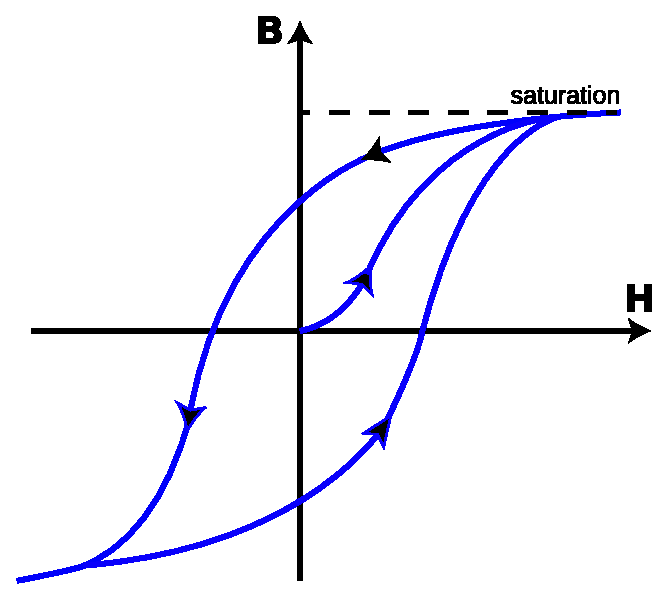
\includegraphics[width=2.5in]{modules/m0058_HysteresisSVG_se170826.eps}
% https://commons.wikimedia.org/wiki/File:HysteresisSVG.svg (modified)
}}{A two dimensional plane labeled H (vertical) - B (horizontal) plane. A blue feather like shape is shown in the plane made of 3 blue lines. At an arbitrary point on B extends a perpendicular, dashed line labeled saturation. One line is shown starting at the origin, increasing in a curve and gradually flattening at the saturation line. From that intersection point the left line increases in a negative direction through the second and third quadrants gradually flattening. The third line is a mirror image of the second line and increases from the third quadrant and gradually flattens at the saturation line.}
\end{center} 
\centerline{\scriptsize 
\copyright~\hyperref[m0058_fMatSatHys_Credit]{Ndthe} (modified)
\href{https://creativecommons.org/licenses/by-sa/3.0/deed.en}{CC BY~SA 3.0} 
} 
\caption{
\label{m0058_fMatSatHys}
Non-linearity in a ferromagnetic material manifesting as saturation and hysteresis.
}
\end{figure}

Once the external magnetizing field ${\bf H}$ exceeds a certain value, the response field ${\bf B}$ no longer significantly increases.
This is saturation. 
Once saturated, further increases in the external field result do not significantly increase the magnetization of the material, so there is no significant increase in ${\bf B}$. 

From this state of saturation, let us now reduce the external field.
We find that the rate of decrease in ${\bf B}$ with respect to ${\bf H}$ is significantly less than the rate that ${\bf B}$ originally increased with respect to ${\bf H}$.
In fact, ${\bf B}$ is still greater than zero even when ${\bf H}$ has been reduced to zero.
At this point, the magnetization of the material is obvious, and a device comprised of this material could be used as a magnet.

If we now apply an external field in the reverse direction, we find that we are eventually able to zero and then redirect the response field.
As we continue to decrease ${\bf H}$ (that is, increase the magnitude in the reverse direction), we once again reach saturation.

The same behavior is observed when we once again increase ${\bf H}$.  The material is eventually demagnetized, remagnetized in the opposite direction and then saturated in that direction.
At this point, it is apparent that a return to the start condition (${\bf H}={\bf B}=0$; i.e., demagnetized when there is no external field) is not possible.

Hysteresis is the name that we apply to this particular form of non-linear behavior.
Hysteresis has important implications in engineering applications.
First, as identified above, it is an important consideration in the analysis and design of magnets.
In applications where a ferromagnetic material is being used because high permeability is desired -- e.g., in inductors 
\index{inductor!hysteresis}
(Section~\ref{m0123_Inductance}) and transformers (Section~\ref{m0031_Transformers_Principle_of_Operation}) 
\index{transformer!hysteresis}
-- hysteresis complicates the design and imposes limits on the performance of the device.

\emph{Hysteresis} 
\index{hysteresis}
may also be exploited as a form of memory.
This is apparent from Figure~\ref{m0058_fMatSatHys}.
If ${\bf B}>0$, then recent values of ${\bf H}$ must have been relatively large and positive.  Similarly,
If ${\bf B}<0$, then recent values of ${\bf H}$ must have been relatively large and negative.
Furthermore, the most recent sign of ${\bf H}$ can be inferred even if the present value of ${\bf H}$ is zero.
In this sense, the material ``remembers'' the past history of its magnetization and thereby exhibits memory.
This is the enabling principle for a number of digital data storage devices, including hard drives (see ``Additional Reading'' at the end of this section).
Summarizing:
%
%ORB HIGHLIGHT
\begin{mdframed}[backgroundcolor=yellow!20,nobreak=true] 
Ferromagnetic media exhibit permeability $\mu$ that is orders of magnitude greater than that of free space and are readily magnetizable.  
These materials are also nonlinear in $\mu$, which manifests as saturation and hysteresis.
\end{mdframed}

%%%%%%%%%%%%%%%%%%%%%%%%%%%%%%%%%%%%%%%%

{\bf Additional Reading:}
\begin{itemize}
\item Section~\ref{m0136_Table_of_Permeabilities} (``Permeability of Some Common Materials'')
\item ``\href{https://en.wikipedia.org/wiki/Magnetism}{Magnetism}'' on Wikipedia.
\item ``\href{https://en.wikipedia.org/wiki/Ferrite_(magnet)}{Ferrite (magnet)}'' on Wikipedia.
\item ``\href{https://en.wikipedia.org/wiki/Paramagnetism}{Paramagnetism}'' on Wikipedia.
\item ``\href{https://en.wikipedia.org/wiki/Diamagnetism}{Diamagnetism}'' on Wikipedia.
\item ``\href{https://en.wikipedia.org/wiki/Ferromagnetism}{Ferromagnetism}'' on Wikipedia.
\item ``\href{https://en.wikipedia.org/wiki/Magnetic_hysteresis}{Magnetic hysteresis}'' on Wikipedia.
\item ``\href{https://en.wikipedia.org/wiki/Magnetic_storage}{Magnetic storage}'' on Wikipedia.
\item ``\href{https://en.wikipedia.org/wiki/Hard_disk_drive}{Hard disk drive}'' on Wikipedia.
\end{itemize}

\index{materials, magnetic|)}
\index{materials (properties)|)}
